%% Los cap'itulos inician con \chapter{T'itulo}, estos aparecen numerados y
%% se incluyen en el 'indice general.
%%
%% Recuerda que aqu'i ya puedes escribir acentos como: 'a, 'e, 'i, etc.
%% La letra n con tilde es: 'n.


\chapter{Resultados}

\section{Paquete de R \emph{geneticae}}

El paquete \emph{geneticae} permite analizar datos provenientes de etapas avanzadas de los programas de mejoramiento, donde se evalúan pocos genotipos en diversos ambientes. 

Una vez instalado el paquete, se debe cargar en la sesion de R mediante el comando: \textcolor{blue}{library}(geneticae). Información detallada sobre las funciones del paquete geneticae se puede obtener mediante \textcolor{blue}{help}(package = ``geneticae"). La ayuda para una función, por ejemplo \textcolor{blue}{imputation}(), en una sesión R se puede obtener usando \emph{?imputation} o \textcolor{blue}{help}(imputation). Además, a partir de la función \textcolor{blue}{browseVignettes}(``geneticae") se obtiene la viñeta del paquete, es decir una descripción el problema que está diseñado para resolver asi como ejemplos de aplicación del mismo.

\subsection{Conjuntos de datos en geneticae}

El paquete geneticae proporciona dos conjuntos de datos que permiten ilustrar la metodología incluida para analizar los datos obtenidos de EMA.
\begin{itemize}[wide, nosep, labelindent = 0pt, topsep = 1ex, noitemsep,topsep=0pt]
\item \emph{yan.winterwheat dataset}: rendimiento de 18 variedades de trigo de invierno cultivadas en nueve ambientes en Ontario en 1993. A pesar de que el experimento contaba con cuatro bloques o réplicas en cada ambiente en el conjunto de datos, obtenido del paquete agridat (Wright, 2018), sólo el rendimiento medio por variedad se encuentra disponible.
\begin{tcolorbox}[skin=bicolor,
    colframe=aurometalsaurus,colback=backcolour,colbacklower=white,
    width=1\linewidth,
    height=0.4\linewidth,
    boxsep=-3mm]
\begin{lstlisting}[linewidth=\columnwidth]
data(yan.winterwheat)
yanwinterwheat <- yan.winterwheat
head(yanwinterwheat)
\end{lstlisting}

\tcblower\vskip-\baselineskip
\tcblower
\vspace{0.5cm}
\footnotesize\begin{verbatim}
##   gen  env yield
## 1 Ann BH93 4.460
## 2 Ari BH93 4.417
## 3 Aug BH93 4.669
## 4 Cas BH93 4.732
## 5 Del BH93 4.390
## 6 Dia BH93 5.178
\end{verbatim}
\end{tcolorbox}

\item \emph{plrv dataset}: Estudio de resistencia a PLRV (\emph{Patato Leaf Roll Virus}) causante del enrollamiento de la hoja. Se experimentaron 28 genotipos en 6 ubicaciones en Perú. Cada clon fue evaluado tres veces en cada ambiente, y de cada uno de ellos se contaba con el rendimiento, peso de planta y parcela. Este conjunto de datos se obtuvo del paquete agricolae.\\

\begin{tcolorbox}[skin=bicolor,
    colframe=aurometalsaurus,colback=backcolour,colbacklower=white,
    width=1\linewidth,
    height=0.4\linewidth,
    boxsep=-3mm]
\begin{lstlisting}
data(plrv)
plrv <- plrv
head(plrv)
\end{lstlisting}

\tcblower\vskip-\baselineskip
\tcblower
\vspace{0.5cm}
\footnotesize\begin{verbatim}
##   Genotype Locality Rep WeightPlant WeightPlot    Yield
## 1   102.18     Ayac   1   0.5100000       5.10 18.88889
## 2   104.22     Ayac   1   0.3450000       2.76 12.77778
## 3   121.31     Ayac   1   0.5425000       4.34 20.09259
## 4   141.28     Ayac   1   0.9888889       8.90 36.62551
## 5   157.26     Ayac   1   0.6250000       5.00 23.14815
## 6    163.9     Ayac   1   0.5120000       2.56 18.96296
\end{verbatim}
\end{tcolorbox} 
\end{itemize}
  
\subsection{Aplicación de las funciones incluidas en el paquete}

A fin de ilustrar la metodología incluida en el paquete se utiliza el conjunto de datos \emph{yan.winterwheat} a modo de ejemplo.\\


\textbf{GGE biplot}

Para visualizar conjuntamente el efecto de G y IGA Yan et al. (2000) propuso el biplot GGE, con el cual se pueden abordar visualmente diversos aspectos relacionados con la evaluación de genotipos y ambientes. Para obtener dicho biplot en primer lugar se debe ajustar el modelo SREG mediante la función \textcolor{blue}{GGEmodel}(). Esta función es menos restrictiva que las disponibles actualmente en R en cuanto al conjunto de datos de entrada. En particular, es una modificación de la  función \textcolor{blue}{GGEModel}() del paquete GGEBiplots \textbf{(CITA)} el cual requiere que en el conjunto de datos de entrada los genotipos se encuentren en las filas y los ambientes en las columnas, es decir que no admiten replicas. En este caso, el conjunto de datos de entrada de \textcolor{blue}{GGEmodel}() debe estar en formato largo, lo cual es más ordenado a la hora de registrar la información \textbf{(CITA)}. Esto significa que las observaciones se encuentran en las filas y variables, genotipos, ambientes, repeticiones (en caso de que haya) y el fenotipo observado, en las columnas. Además puede incluir otras variables que no serán utilizadas en el análisis ya que al ajustar el modelo se deben indicar los nombres de las variables a emplear. Por otro lado, si cada genotipo ha sido evaluado más de una vez en cada ambiente, la función calcula automáticamente el valor fenotípico promedio para cada combinación de genotipo y ambiente para luego ajustar el modelo. Los valores faltantes no están permitidos, en caso de haber, un mensaje de error saldrá en la consola de R.\\  
\begin{tcolorbox}[colframe=aurometalsaurus,colback=backcolour,colbacklower=white,
   				width=1\linewidth,
    			height=0.1\linewidth,
    			boxsep=-3mm]
\begin{lstlisting}
GGE1 <- GGEmodel(yanwinterwheat, genotype = ``gen", environment = ``env", response = ``yield")
\end{lstlisting}
\end{tcolorbox}
La salida de la función \textcolor{blue}{GGEmodel}() es una lista que contiene las coordenadas para genotipos y ambientes de todas las componentes, el vector de valores propios de cada componente, la variancia total, el porcentaje de variancia explicada por cada componente, entre otros. Utilizando dicha información, la función \textcolor{blue}{GGEPlot}() construye los biplots GGE. En dichos gráficos los cultivares se muestran en minúscula, para diferenciarlos de los ambientes, que están en mayúsculas. La primer componente principal se usa como la abscisa y la segunda como ordenada. Además, es posible adicionar el método de centrado, escala y SVD utilizado, y el porcentaje G + GE explicado por los dos ejes como una nota al pie del biplot con la opción \emph{footnote=T}, así como también el nombre del gráfico con \emph{titles = T}.


En la figura \ref{fig:fig4121} se presenta un biplot básico, el cual explica el 78\% de la variabilidad total de G + GE. 

\begin{tcolorbox}[skin=bicolor,
    colframe=aurometalsaurus,colback=backcolour,colbacklower=white,
    width=1\linewidth,
    height=0.65\linewidth,
    boxsep=-3mm]
\begin{lstlisting}
GGEPlot(GGE1, type = "Biplot", footnote = F, titles = F)
\end{lstlisting}
\tcblower\vskip-\baselineskip
\tcblower
\begin{figure}[H]
	\begin{center}
		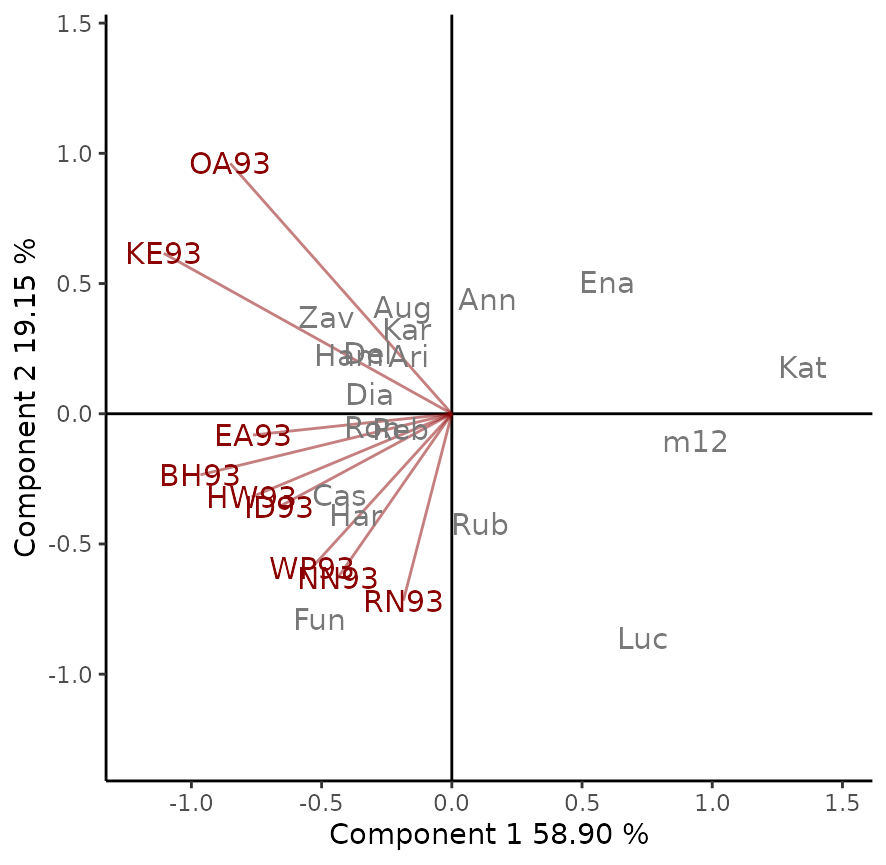
\includegraphics[width=9.5cm]{./Graficos/GGE_BIPLOT.png}
	\end{center}
	\caption{Biplot básico obtenido de la función \textcolor{blue}{GGEPlot}()}
	\label{fig:fig4121}
\end{figure}
\end{tcolorbox} 

Los mejoradores en general están interesados en identificar los cultivares más adaptados a su área. Para identificar los mejores genotipos en un ambiente a través del biplot GGE, Yan y Hunt (2002) sugieren constituir un eje del ambiente, por ejemplo OA93, trazando una recta que pase por el identificador del ambiente y el origen. Los genotipos se pueden clasificar de acuerdo con sus proyecciones en el eje OA93 en función de su rendimiento en dicho ambiente, en la dirección indicada por la flecha (Figura \ref{fig:fig4122}). Por lo tanto, el cultivar de mayor rendimiento fue es Zav seguido por Aug, Ham, y así sucesivamente hasta llegar al genotipo Luc, que es el de rendimiento mas bajo en ese ambiente. La línea que pasa a través del origen de coordenadas y es perpendicular al eje OA93 separa los genotipos que rindieron por encima de la media, de Zav a Cas, de aquellos que rindieron por debajo de la medi,a de Ema a Luc, en OA93.

\begin{tcolorbox}[skin=bicolor,
    colframe=aurometalsaurus,colback=backcolour,colbacklower=white,
    width=1\linewidth,
    height=0.7\linewidth,
    boxsep=-3mm]
\begin{lstlisting}
GGEPlot(GGE1, type = "Selected Environment", selectedE = "OA93", footnote = F, titles = F)
\end{lstlisting}
\tcblower\vskip-\baselineskip
\tcblower
\begin{figure}[H]
	\begin{center}
		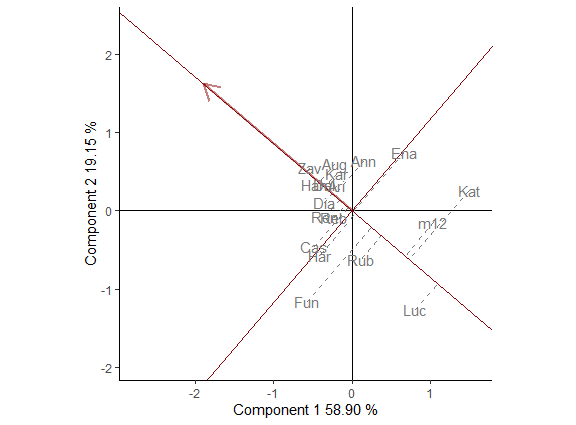
\includegraphics[width=9.5cm]{./Graficos/SelectedEnvironment.png}
	\end{center}
	\caption{Ranking de cultivares para un ambiente determinado obtenido de la función \textcolor{blue}{GGEPlot}()}
	\label{fig:fig4122}
\end{figure}
\end{tcolorbox} 

Otro interes de los fitomejoradores es determinar cuál es el ambiente más adecuado para un cultivar. La figura \ref{fig:fig4123} ilustra cómo visualizar la adaptación relativa del cultivar Luc en diferentes ambientes. Yan y Hunt (2002) sugieren graficar una línea que una el origen de coordenadas y el marcador de Luc, el cual llamaremos eje Luc. Los ambientes se clasifican a lo largo del eje Luc en la dirección indicada por la flecha. La línea que pasa por el origen y es perpendicular al eje de Luc separa los ambientes en los que Luc presentó un rendimiento por debajo de su promedio, OA93 a ID93, de aquellos en los que rindió por encima de la media, RN93 a WP93.
\begin{tcolorbox}[skin=bicolor,
    colframe=aurometalsaurus,colback=backcolour,colbacklower=white,
    width=1\linewidth,
    height=0.65\linewidth,
    boxsep=-3mm]
\begin{lstlisting}
GGEPlot(GGE1, type = "Selected Genotype", selectedG = "Luc", footnote = F, titles = F)
\end{lstlisting}
\tcblower\vskip-\baselineskip
\tcblower
\begin{figure}[H]
	\begin{center}
		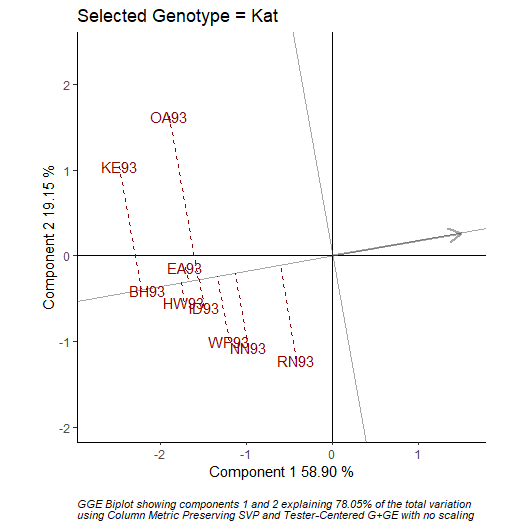
\includegraphics[width=9.5cm]{./Graficos/SelectedGenotype.png}
	\end{center}
	\caption{Ranking de ambientes para cultivar determinado obtenido de la función \textcolor{blue}{GGEPlot}()}
	\label{fig:fig4123}
\end{figure}
\end{tcolorbox} 


Para comparar dos cultivares, por ejemplo Rub y Zav, se propone unir mediante una línea recta los genotipos a comparar, luego trazar una línea que pase por el origen y que sea perpendicular a la línea que une a los genotipos. (figura \ref{fig:fig4124}). Se observa que tres ambientes, RN93, NN93 y WP93, se encuentran del mismo lado de la línea perpendicular que Rub, y los otros seis ambientes están en el otro lado de la línea perpendicular, junto el marcador del cultivar Zav. Esto indica que Rub fue mas rendidor que Zav en RN93, NN93 y WP93, pero Zav fue superior a Rub en los seis ambientes restantes.


\begin{tcolorbox}[skin=bicolor,
    colframe=aurometalsaurus,colback=backcolour,colbacklower=white,
    width=1\linewidth,
    height=0.65\linewidth,
    boxsep=-3mm]
\begin{lstlisting}
GGEPlot(GGE1, type = "Comparison of Genotype", selectedG1 = "Rub", selectedG2 = "Zav", footnote = F, titles = F)
\end{lstlisting}
\tcblower\vskip-\baselineskip
\tcblower
\begin{figure}[H]
	\begin{center}
		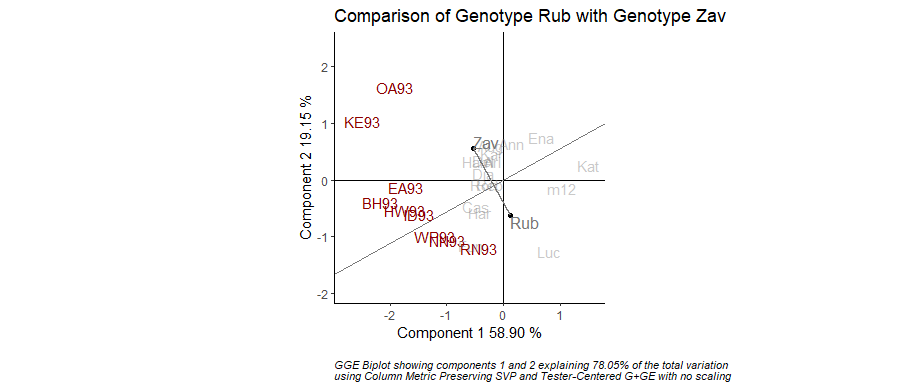
\includegraphics[width=9.5cm]{./Graficos/ComparisonofGenotype.png}
	\end{center}
	\caption{Comparación entre dos genotipos obtenido de la función \textcolor{blue}{GGEPlot}()}
	\label{fig:fig4124}
\end{figure}
\end{tcolorbox}


La vista poligonal del biplot GGE, documentado por primera vez en Yan (1999), proporciona un medio eficaz de visualización del patrón ``quíen ganó dónde" de un conjunto de datos EMA (Figura \ref{fig:fig4125}). 
El polígono se dibuja uniendo los cultivares (fun, zav, ena, kat y luc) que se encuentran más alejados del origen de coordenadas, de modo que todos los cultivares se encuentren contenidos en el polígono. Los cultivares de vértice son aquellos con  vectores más largos, en sus respectivas direcciones, la cual es una medida de la capacidad de respuesta a los ambientes. 

Las líneas perpendiculares a los lados del polígono dividen el biplot en megaambientes, cada uno de ellos tiene un cultivar de vértice, el de mayor rendimiento en todos los ambientes que se encuentran en él. Por un lado, se observa que OA93 y KE93 se encuentran en el mismo sector y que Zav es el mejor cultivar. Otro sector esta formado por el resto de los ambientes, siendo Fun el cultivar que se encuentra en el vertice de dicho sector. En los sectores con ena, kat y luc en los vértices no se observó ningun ambiente. Esto indica que estos cultivares fueron los menos rendidores en algunos o todos los ambientes considerados.

Se requieren dos criterios para sugerir la existencia de diferentes megaambientes (Gauch and Zobel, 1997). Primero, diferentes variedades superiores en los diferentes ambientes estudiados; en segundo lugar, la variación entre grupos debería ser significativamente mayor que la variación dentro del grupo.  Ambos criterios se cumplen en el presente caso (Figura \ref{fig:fig4125}). La sugerencia de dos megaambientes coincide con la distribución geográfica de los ambientes. La ubicación de OA (Ottawa) y KE (Kemptville) se extiende hacia el este de Ontario; BH (Bath) también pertenece al este de Ontario, pero es mucho más cálido que OA y KE. Los otros seis lugares pertenecen al oeste o sur de la provincia.

\begin{tcolorbox}[skin=bicolor,
    colframe=aurometalsaurus,colback=backcolour,colbacklower=white,
    width=1\linewidth,
    height=0.65\linewidth,
    boxsep=-3mm]
\begin{lstlisting}
GGEPlot(GGE1, type = "Which Won Where/What", footnote = F, titles = F)
\end{lstlisting}
\tcblower\vskip-\baselineskip
\tcblower
\begin{figure}[H]
	\begin{center}
		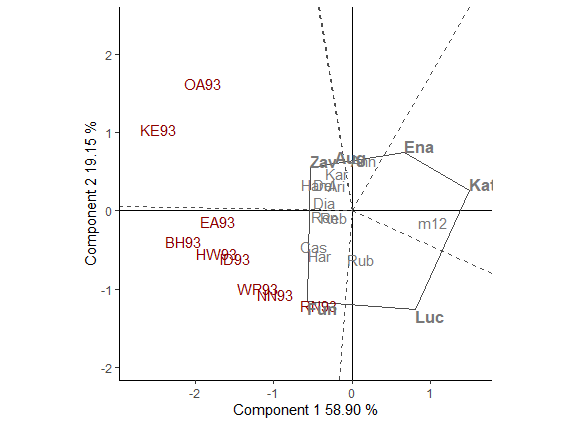
\includegraphics[width=9.5cm]{./Graficos/WhichWonWhereWhat.png}
	\end{center}
	\caption{Identificación del mejor cultivar en cada ambiente a partir de la función \textcolor{blue}{GGEPlot}()}
	\label{fig:fig4125}
\end{figure}
\end{tcolorbox}




Otro interés entre los fitomejoradores es seleccionar cultivares dentro de cada uno de los mega-ambientes definidos. De acuerdo con la figur  \ref{fig:fig4125}, zav es el mejor cultivar para los ambientes en uno de los mega-ambiente y fun en el otro. Sin embargo, los mejoradores no seleccionarán un único cultivar en cada mega-ambiente, sino que es necesario observar en más detalle cada mega-ambiente y evaluar todos los cultivares con el fin de obtener una idea de su desempeño (rendimiento y estabilidad).
El GGE biplot, particularmente su forma de escalado centrada en el genotipo, proporciona un medio superior para visualizar tanto el rendimiento medio como la estabilidad de los genotipos. La visualización del rendimiento medio y la estabilidad de los genotipos se logra a partir de una coordenada de medio ambiente en el biplot centrado en el genotipo (Figura \ref{fig:fig4126}). La abscisa representa el efecto de G mientras que la ordenada la IGA asociada con cada genotipo, que es una medida de la variabilidad o inestabilidad de los genotipos. Una mayor proyección sobre la ordenada AEC, independientemente de la dirección, significa mayor inestabilidad. Por lo tanto, rub y dia son más variables y menos estables que otros cultivares (Figura \ref{fig:fig4126}). El ambiente BH93 está ubicado en el este de Ontario caracterizado por inviernos más fríos, mientras que RN93 en el sur de Ontario caracterizado por un clima cálido y húmedo en la mayoría de los años. Esto justifica la inestabilidad de rub y dia, ya que el primero es temprano y tiene una poca resistencia al invierno por lo que se desempeñó bien en RN93 y mal en BH93, y el segundo, con un comportamiento contrario al anterior cultivar debido a que es tardío y alto. Los cultivares próximos al eje de las abscisas, cas, zav, reb, del, ari y kar, son más estables que el resto. 

\begin{tcolorbox}[skin=bicolor,
    colframe=aurometalsaurus,colback=backcolour,colbacklower=white,
    width=1\linewidth,
    height=0.65\linewidth,
    boxsep=-3mm]
\begin{lstlisting}
GGEPlot(GGE1, type = "Mean vs. Stability", footnote = F, titles = F)
\end{lstlisting}
\tcblower\vskip-\baselineskip
\tcblower
\begin{figure}[H]
	\begin{center}
		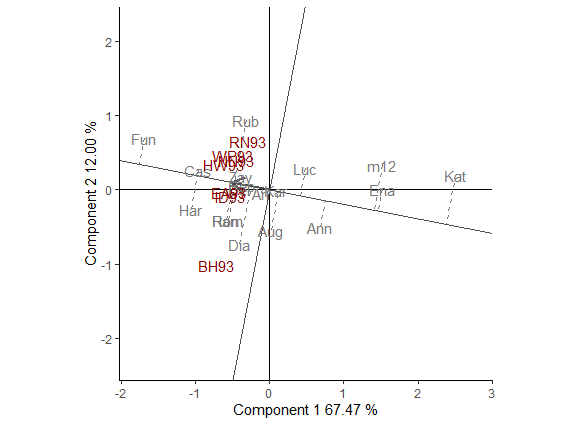
\includegraphics[width=9.5cm]{./Graficos/MeanvsStability.png}
	\end{center}
	\caption{Evaluación de los cultivares con base en el rendimiento promedio y la estabilidad a partir de la función \textcolor{blue}{GGEPlot}()}
	\label{fig:fig4126}
\end{figure}
\end{tcolorbox}

El biplot GGE permite visualizar tanto el rendimiento medio como la estabilidad de los genotipos en la unidad de rendimiento per se. Ésto permite que las dos medidas se combinen y visualicen en una sola medida (Figura \ref{fig:fig4127}). El pequeño círculo en la figura \ref{fig:fig4127} representa el cultivar ideal ya que es el más rendidor del conjunto de datos y es absolutamente estable, al estar ubicado en el eje de abscisa del AEC. Tal genotipo ideal se utiliza como referencia para la evaluacion de los cultivares ya que rara vez es exista. La distancia entre los cultivares con respecto al ideal se puede utilizar como una medida de su conveniencia. Los círculos concéntricos, tomando el cultivar ideal como centro, ayudan a visualizar la distancia entre todos los cultivares y el ideal. El cultivar fun es el más próximo al ideal, y por lo tanto, el más deseable de todos los cultivares probados, seguido por cas y heno, que a su vez son seguidos por ron, ham, rub, zav, del y reb, etc.



\begin{tcolorbox}[skin=bicolor,
    colframe=aurometalsaurus,colback=backcolour,colbacklower=white,
    width=1\linewidth,
    height=0.65\linewidth,
    boxsep=-3mm]
\begin{lstlisting}
GGEPlot(GGE1, type = "Ranking Genotypes", footnote = F, titles = F)
\end{lstlisting}
\tcblower\vskip-\baselineskip
\tcblower
\begin{figure}[H]
	\begin{center}
		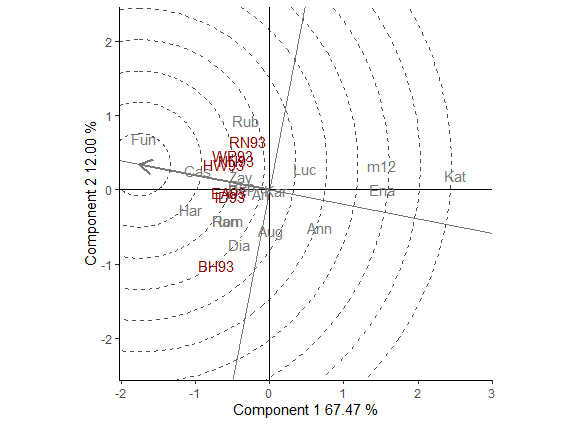
\includegraphics[width=9.5cm]{./Graficos/RankingGenotypes.png}
	\end{center}
	\caption{Clasificación de genotipos con respecto al genotipo ideal a partir de la función \textcolor{blue}{GGEPlot}()}
	\label{fig:fig4127}
\end{figure}
\end{tcolorbox}


A pesar de que los EMA se realizan para evaluar cultivares, son igualmente útiles para evaluar los ambientes estudiados. Ésto incluye diversos aspectos: (i) evaluar si la región objetivo pertenece a uno o varios megaambientes; (ii) identificar mejores ambientes de prueba; (iii) identificar ambientes redundantes que no brindan información adicional sobre los cultivares; (iv) identificar ambientes que pueden usarse para la selección indirecta.

En la figura \ref{fig:fig4128} se observa que los ambientes estan conectados con el origen de coordenadas a través de vectores, permitiendo comprender las interrelaciones entre los distintos ambientes. El coseno del ángulo entre los vectores de dos ambientes se aproxima al coeficiente de correlación entre ellos. Por ejemplo, NN93 y WP93 tienen un ángulo de aproximadamente $10^{\circ}$ entre sus vectores; por lo tanto, se encuentran estrechamente relacionados; mientras que RN93 y OA93 presentan correlaciones leves y negativas ya que el ángulo supera los $90^{\circ}$. El coseno de los ángulos no se traduce con precisión en coeficientes de correlación, ya que el biplot no explica toda la variación en el conjunto de datos. Sin embargo, los ángulos son lo suficientemente informativos como para permitir una imagen completa sobre la interrelación entre el entorno de prueba.

Por otro lado, la Figura \ref{fig:fig4129} ayuda a identificar ambientes redundantes. Si algunos de los ambientes tienen ángulos pequeños y, por lo tanto, están altamente correlacionados, la información sobre los genotipos obtenidos de estos ambientes debe ser similar. Si esta similitud es repetible a través de los años, estos ambientes son redundantes y por lo tanto, uno solo debería ser suficiente. Obtener la misma o mejor información utilizando menos ambientes reducirá el costo y aumentará la eficiencia de producción.

\begin{tcolorbox}[skin=bicolor,
    colframe=aurometalsaurus,colback=backcolour,colbacklower=white,
    width=1\linewidth,
    height=0.65\linewidth,
    boxsep=-3mm]
\begin{lstlisting}
GGEPlot(GGE1, type = "Relationship Among Environments", footnote = F, titles = F)
\end{lstlisting}
\tcblower\vskip-\baselineskip
\tcblower
\begin{figure}[H]
	\begin{center}
		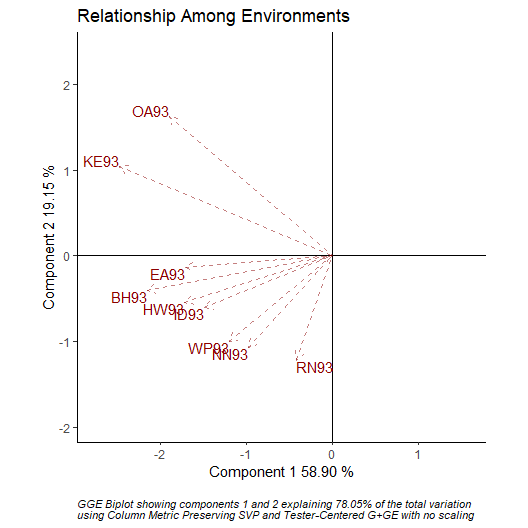
\includegraphics[width=9.5cm]{./Graficos/RelationshipAmongEnvironments.png}
	\end{center}
	\caption{Relación entre ambientes obtenido de la función \textcolor{blue}{GGEPlot}()}
	\label{fig:fig4128}
\end{figure}
\end{tcolorbox}


La capacidad de discriminación es una medida importante de un ambiente, ya que si no tiene dicha capacidad no proporciona información sobre los cultivares y, por lo tanto, el ambiente carece de utilidad. Otra medida igualmente importante de un ambiente es su representatividad del ambiente objetivo, ya que si no es representativo no solo que carece de utilidad sino que también puede proporcionar información sesgada sobre los cultivares evaluados

La representatividad de un ambiente es difícil de medir, ya que no es posible muestrear todos los ambientes posibles dentro de un megaambiente y, posteriormente, determinar la representatividad de cada uno en forma individual. Mediante el biplot, la manera de medir la representatividad es definir un entorno promedio y usarlo como referencia. El ambiente promedio está indicado por el círculo pequeño en la figura \ref{fig:fig4129}. El ángulo entre el vector de un ambiente y el eje que pasa a través del origen biplot y el ambiente promedio es una medida de la representatividad del ambiente. Por lo tanto, EA93 e ID93 son los más representativos, mientras que RN93 y BH93 son los menos representativos del ambiente promedio, cuando se analiza el mega-ambiente que no contiene a OA93 y a KE93.

Un ambiente de prueba ideal debe ser tanto discriminatorio como representativo. La figura \ref{fig:fig4129}, utiliza el ambiente ideal como el centro de un conjunto de circulos concéntricos que sirven como regla para medir la distancia entre un ambiente y el ideal. HW93 es el ambiente más cercano al ideal y, por lo tanto, es el más deseable de los siete entornos, es seguido por EA93 e ID93, que a su vez son seguidos por WP93 y NN93. RN93 y BH93 fueron los ambientes de prueba menos deseable. Además, EA93 e ID93, y NN93 y WP93 son pares de entornos muy similares, lo cual tambien se visualizó que se pueden visualizar mejor desde la figura. Anterior


figu \ref{fig:fig4129}
\begin{tcolorbox}[skin=bicolor,
    colframe=aurometalsaurus,colback=backcolour,colbacklower=white,
    width=1\linewidth,
    height=0.65\linewidth,
    boxsep=-3mm]
\begin{lstlisting}
GGEPlot(GGE1, type = "Ranking Environments", footnote = F, titles = F)
\end{lstlisting}
\tcblower\vskip-\baselineskip
\tcblower
\begin{figure}[H]
	\begin{center}
		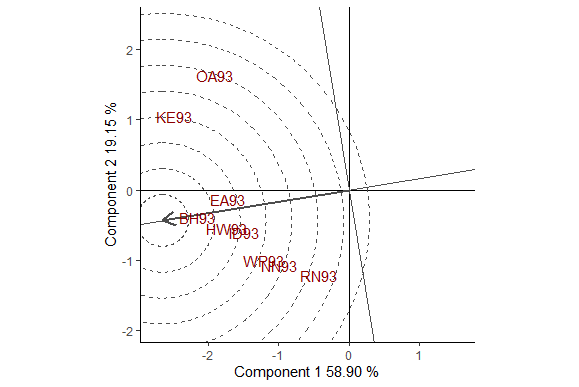
\includegraphics[width=9.5cm]{./Graficos/RankingEnvironments.png}
	\end{center}
	\caption{Clasificación de ambientes con respecto al ambiente ideal a partir de la función \textcolor{blue}{GGEPlot}()}
	\label{fig:fig4129}
\end{figure}
\end{tcolorbox}



\textbf{Falta un grafico q es discriminacion vs representatividad q no se como se interpreta....}

\textbf{Biplot GE}


Para visualizar solamente el efecto de IGA se utilizan los biplots GE obtenidos del modelo AMMI. Para ejecutar la función \textcolor{blue}{rAMMI}(), siendo el formato del conjunto de datos requerido igual al descripto para la función \textcolor{blue}{GGEmodel}(). Sin embargo, en este caso la salida de la función es el biplot GE. Esta función no se encuentra disponible actualmente en R, es modificada de la publicación de Rodrigues et al. (2015). Esta versión de la función permite incluir otras variables en el conjunto de datos debido a que, al igual que en \textcolor{blue}{GGEmodel}(), se deben indicar los nombres de las variables a emplear y además permite la presencia de repeticiones ya que la función calcula automáticamente el valor fenotípico promedio para cada combinación de genotipo y ambiente para luego ajustar el modelo. Los valores faltantes no están permitidos, en caso de haber, un mensaje de error saldrá en la consola de R.\\ 


El biplot clásico para el conjunto de datos \emph{yan.winterwheat} se muestra en la figura \ref{fig:fig41211} junto con la sentencia utlizada para obtener el mismo. Se observa que la magnitud de los vectores de los ambientes BH93, KE93 y OA93 es mayor a la de los demás ambientes, es decir que son los que más contribuyen a la interacción. La cercanía de los marcadores de los genotipos m12 y Kat indica que esos genotipos tienen patrones de interacción similares, y a la vez, muy distintos a los de los genotipos Ann y Aug. Del biplot también se destacan las cercanías entre el genotipo dia y el ambiente BH93 lo que indica, debido a la gran distancia al origen, una fuerte asociación positiva entre el genotipos y el ambientes, es decir, es un ambiente muy favorable para ese genotipo.
Entre las altas asociaciones negativas se puede mencionar a la del ambiente OA93 con el genotipo Luc (marcadores opuestos en el biplot) y se interpreta que ese ambiente es considerablemente desfavorable para ese genotipo. También se observa que los genotipos Cas y Reb están próximos al origen, lo que quiere decir que se adaptan en igual medida a todos los ambientes.


\begin{tcolorbox}[skin=bicolor,
    colframe=aurometalsaurus,colback=backcolour,colbacklower=white,
    width=1\linewidth,
    height=0.7\linewidth,
    boxsep=-3mm]
\begin{lstlisting}
rAMMI(yanwinterwheat, genotype = "gen", environment = "env", response = "yield", type = "AMMI")
\end{lstlisting}
\tcblower\vskip-\baselineskip
\tcblower
\begin{figure}[H]
	\begin{center}
		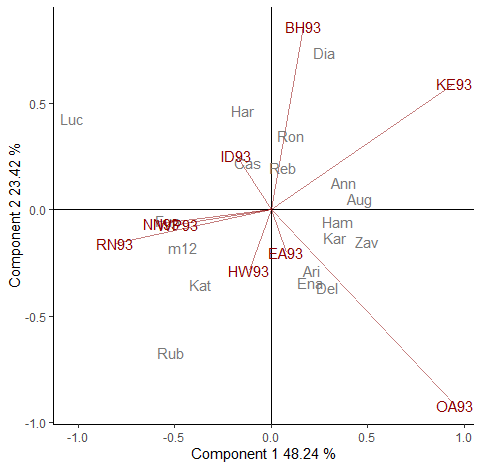
\includegraphics[width=8cm, height=7.6cm]{./Graficos/AMMI.png}
	\end{center}
	\caption{Biplot GE obtenido del modelo clasico AMMI}
	\label{fig:fig41211}
\end{figure}
\end{tcolorbox}



En caso de contar con observaciones atípicas se debe recurrir al biplot obtenido de algunos de los cinco modelos AMMI robustos propuestos por Rodrigues et al. (2015) utilizando la función \textcolor{blue}{rAMMI}().

El conjunto de datos \emph{yan.winterwheat} no presentan observaciones diferentes del resto. Dado que según Rodrigues, et al. (2015) las conclusiones obtenidas con los biplots robustos no serán muy diferentes de las realizadas con el biplot clásico, siendo el modelo rAMMI el que proporciona resultados más similares seguidos por el hAMMI(), carece de sentido interpretar dichos biplots en este ejemplo.

El biplot proveniente de alguno de los modelos robustos se puede obtener mediante la función \textcolor{blue}{rAMMI}() indicando en la opción \emph{type} cuál de ellos se desea obtener: ``rAMMI", ``hAMMI", ``gAMMI", ``lAMMI", ``ppAMMI".


\begin{tcolorbox}[skin=bicolor,
    colframe=aurometalsaurus,colback=backcolour,colbacklower=white,
    width=1\linewidth,
    height=0.1\linewidth,
    boxsep=-3mm]
\begin{lstlisting}
rAMMI(yanwinterwheat, genotype = "gen", environment = "env", response = "yield", type = "rAMMI")
\end{lstlisting}
\end{tcolorbox}



\textbf{Métodos de imputación}

Una limitación importante de los modelos presentados anteriormente es que requieren una que el conjunto de datos este completo, es decir que todos los genotipos sean evaluados en todos los ambientes. Por lo tanto, en el paquete se incluyen una serie de metodologías propuestas, algunas de las cuales no se encuentran disponible en R, para superar el problema de las observaciones perdidas. Entre los métodos incluidos se encuentran: ``EM-AMMI", ``EM-SVD", ``Gabriel",``WGabriel" y ``EM-PCA", los cuales se indican en la opción \emph{type} de la función \textcolor{blue}{imputation}().

\begin{tcolorbox}[skin=bicolor,
    colframe=aurometalsaurus,colback=backcolour,colbacklower=white,
    width=1\linewidth,
    height=0.1\linewidth,
    boxsep=-3mm]
\begin{lstlisting}
imputation(yanwinterwheat, PC.nb = 2, genotype = "gen", environment = "env", response = "yield", type = "EM-AMMI")
\end{lstlisting}
\end{tcolorbox}


\section{Geneticae Shiny Web App}

Generalmente los mejoradores utilizan programas estadísticos que funcionan mediante una interfaz gráfica lo cual permite realizar el análisis de interés sin necesidad del manejo de un lenguaje de programación. \emph{Geneticae Shiny Web App}, es una aplicación web que permite a los usuarios realizar muchos de los análisis incluidos en el paquete geneticae, sin necesidad de conocer el lenguaje de programación R. 

Al iniciar \emph{Geneticae Shiny Web App}, se muestra una pantalla en la cual se carga el conjunto de datos a analizar. Se admiten archivos con extensión .csv, delimitados por coma o punto y coma.
Dado que esta aplicación se conecta con R y utiliza las funciones del paquete \emph{geneticae} se debe respetar el formato requerido por el mismo. El conjunto de datos de entrada debe estar en formato largo, es decir que las observaciones se encuentran en las filas y las variables, genotipos, ambientes, repeticiones (en caso de que haya) y el fenotipo observado, en las columnas. Además puede incluir otras variables que no serán utilizadas en el análisis ya que al cargar el conjunto de datos se debe indicar que columna corresponde al genotipo, al ambiente, a las repeticiones y al valor fenotípico a analizar. La primera fila del conjunto de datos puede contener los nombres de las varibles, y en ese caso se indicará al cargarlo en la aplicación. El número de repeticiones puede diferir con los genotipos y los ambientes.

Dos conjuntos de datos de ejemplo, \emph{plrv} y \emph{yanwinterwheat}, incluidos en el paquete geneticae, se encuentran disponibles en la aplicación para ser descargados y probar la misma (Figura \ref{fig:fig431},\ref{fig:fig432}). La ruta para realizar esto es siguente: \emph{The data} $\rightarrow$ \emph{Example datasets}.

 \begin{figure}[H]
	\begin{center}
		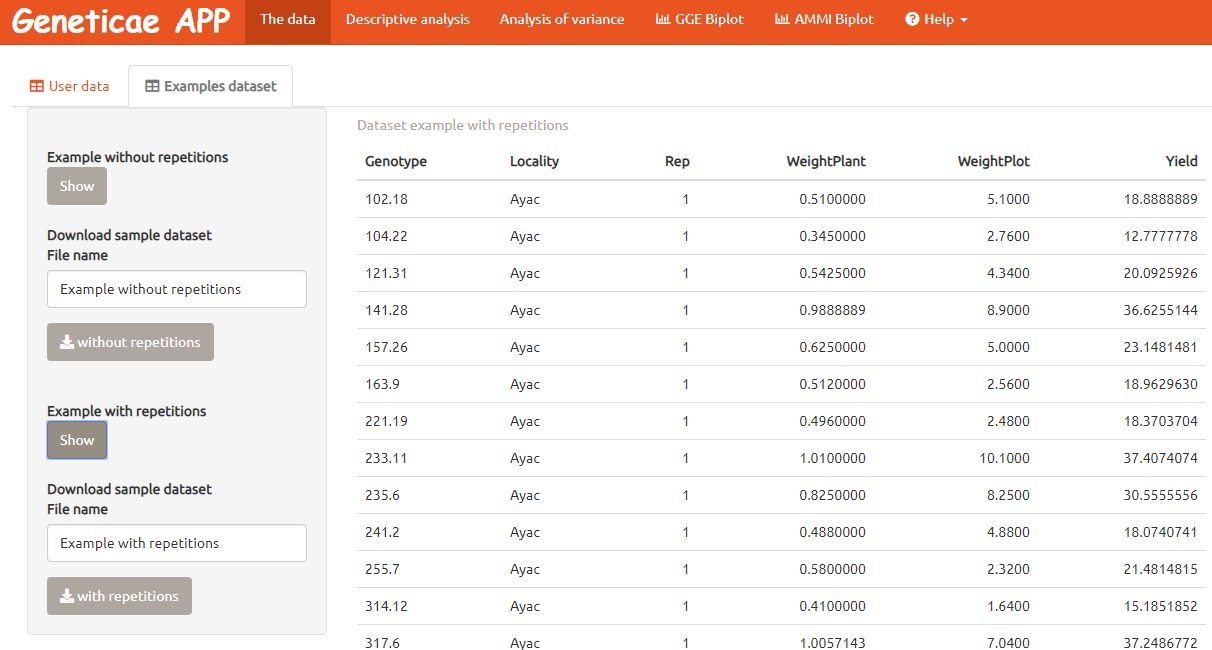
\includegraphics[width=16cm]{./Graficos/Exampledatasets_withoutrep.png}
	\end{center}
	\caption{yanwinterwheat dataset disponible en Shiny Web App}
	\label{fig:fig431}
\end{figure}

\begin{figure}[H]
	\begin{center}
		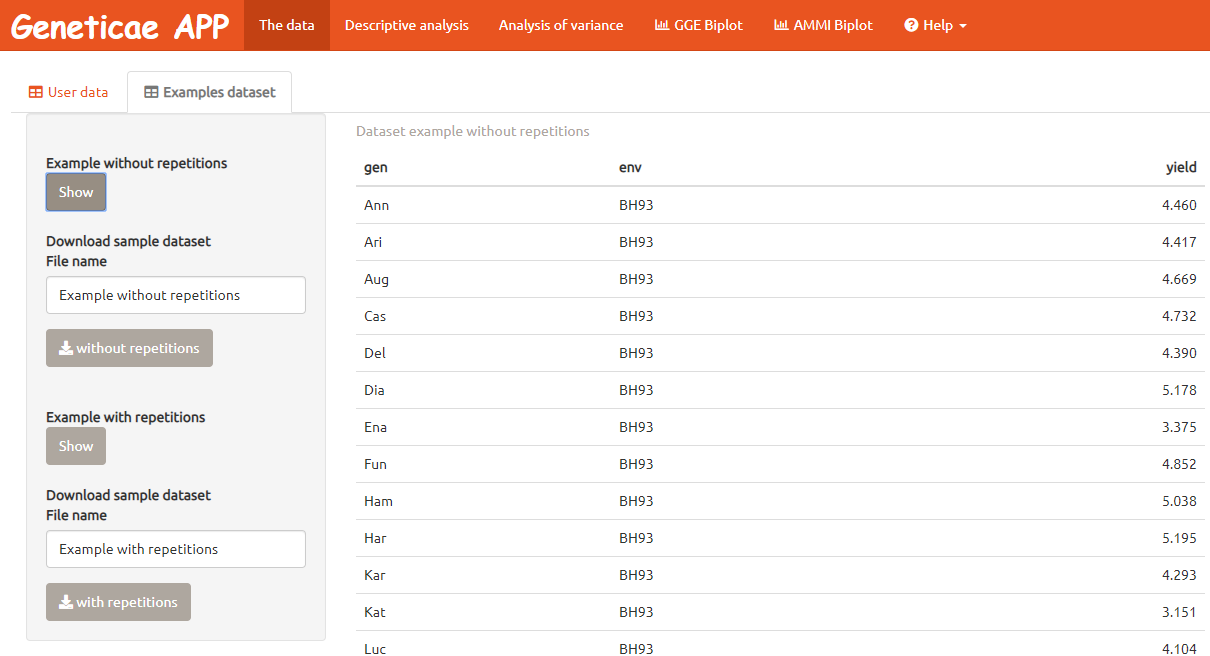
\includegraphics[width=16cm]{./Graficos/Exampledatasets_withrep.png}
	\end{center}
	\caption{plrv dataset disponible en Shiny Web App}
	\label{fig:fig432}
\end{figure}


A fin de ilustrar los diferentes análisis que se pueden realizar con esta aplicación se utiliza el conjunto de datos \emph{yanwinterwheat} (Figura \ref{fig:fig431}). Como se dijo anteriormente, cuenta con información sobre el rendimiento medio de 18 variedades de trigo de invierno cultivadas en nueve ambientes en Ontario en 1993.


\subsection{Análisis de un caso}
En primer lugar se debe importar el conjunto de datos, en este caso \emph{yanwinterwheat}, indicar si el archivo .csv esta delimitado por comas o punto y coma, si la primera fila de encabezado contiene los nombres de cada variable y además, el nombre de la columna que contiene la información de los genotipos, ambientes y valores fenotípicos de interés (Figura \ref{fig:fig433}). En caso de contar con repeticiones, también debe especificarse el nombre de la columna con dicha información.

\begin{figure}[h]
	\begin{center}
		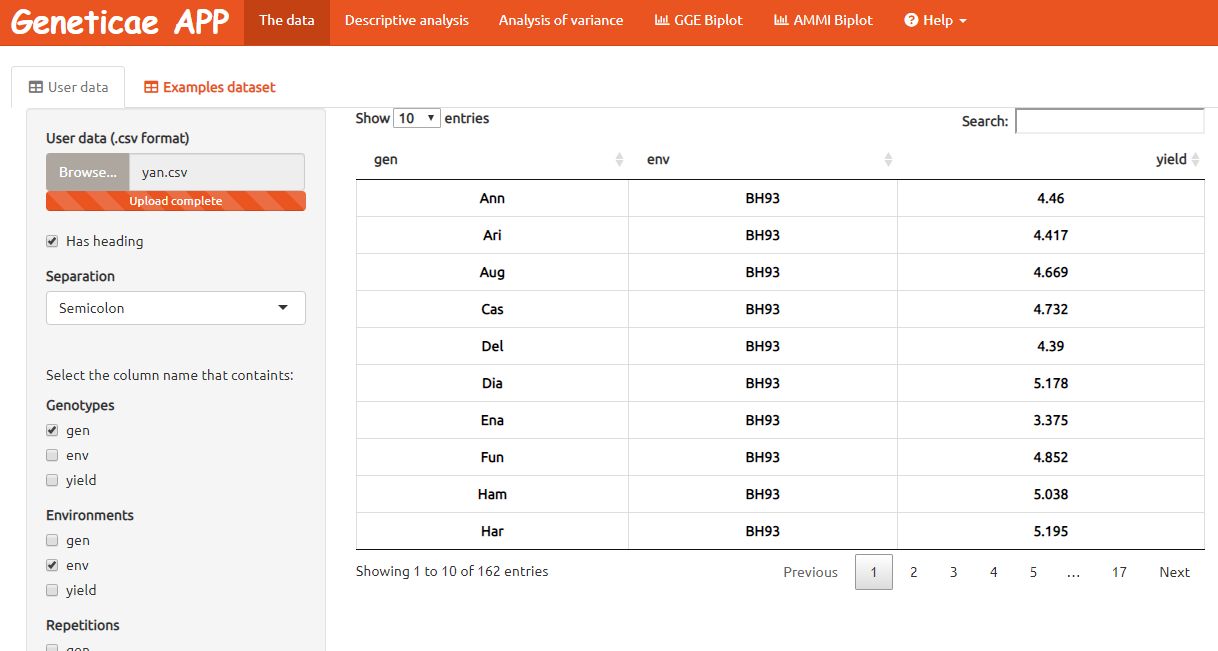
\includegraphics[width=16cm]{./Graficos/data.png}
	\end{center}
	\caption{Importar conjunto de datos}
	\label{fig:fig433}
\end{figure}


\textbf{Análisis descriptivo}

El primer paso de cualquier estudio debe ser un análisis descriptivo del conjunto de datos. La pestaña \emph{Descriptive analysis} brinda diversas herramientas para llevar a cabo dicho análisis. Una de ellas es un boxplot que compara el caracter cuantitativo de interés a través de los ambientes (Figura \ref{fig:figdesc1}) o a través de los genotipos. Este gráfico es interactivo, al posicionarse sobre cada una de las cajas se muestran las medidas resumen utilizadas para la construcción del mismo. Además los mismos se pueden descargar en formato interactivo (.HTML) al hacer click en \emph{Download} así como también en formato .png al hacer click en la cámara que aparece en el gráfico (Figura \ref{fig:figdesc1}). Algunos aspectos del gráfico, como el color de las cajas y los nombres de los ejes, pueden ser personalizados por el usuario. 

\begin{figure}[H]
	\begin{center}
		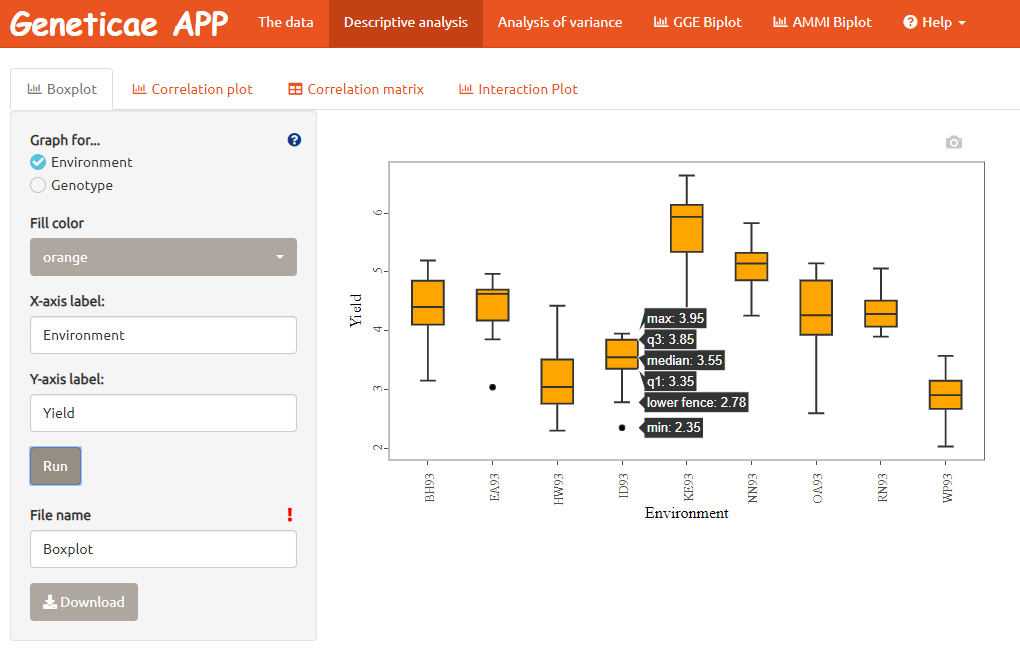
\includegraphics[width=16cm]{./Graficos/Boxplot_environment.png}
	\end{center}
	\caption{Boxplot de ambientes a través de los genotipos para el conjunto de datos Plrv}
	\label{fig:figdesc1}
\end{figure}



Otro interés puede ser estudiar la correlación entre los genotipos o entre los ambientes, para ello tanto el correlograma o gráfico de correlación como la matriz de correlación se pueden realizar (Figura \ref{fig:figdesc2} y \ref{fig:figdesc3}). En ambos casos, se pueden estimar las correlaciones de Pearson o de Spearman. En el correlograma las correlaciones positivas se muestran en azul y las negativas en rojo y la intensidad del color y el tamaño del círculo son proporcionales a los coeficientes de correlación (Figura \ref{fig:figdesc2}). 


\begin{figure}[H]
	\begin{center}
		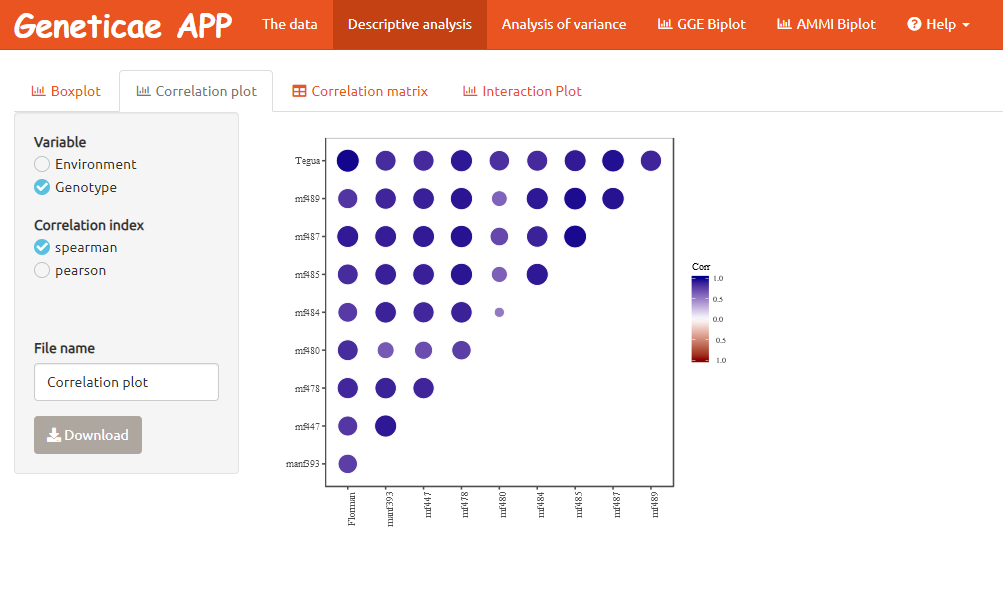
\includegraphics[width=16cm]{./Graficos/corr_gen.png}
	\end{center}
	\caption{Boxplot de genotipos a través de los ambientes para el conjunto de datos Plrv}
	\label{fig:figdesc2}
\end{figure}


\begin{figure}[H]
	\begin{center}
		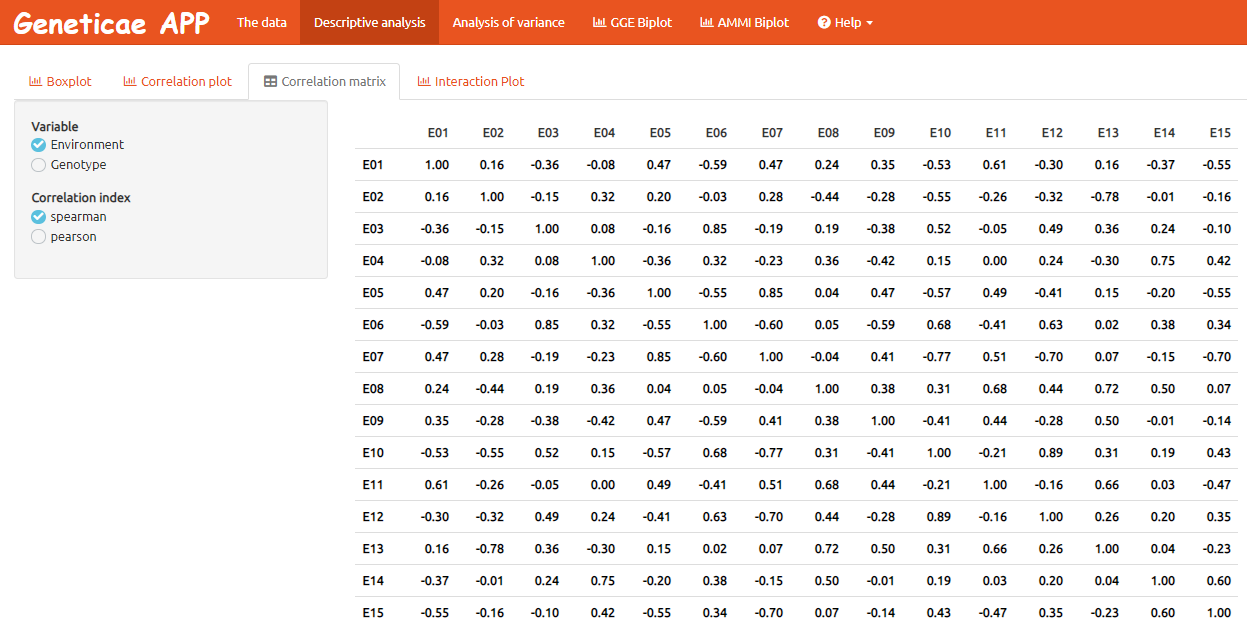
\includegraphics[width=16cm]{./Graficos/corr_matrix.png}
	\end{center}
	\caption{Boxplot de genotipos a través de los ambientes para el conjunto de datos Plrv}
	\label{fig:figdesc3}
\end{figure}



Por último, dado que inconsistencias en el rendimiento de los genotipo en diferentes amientes complican la tarea de los fitomejoradores ya que no existe un genotipo superior en todos los ambientes estudiados y que las técnicas de principal interés de la aplicación carecen de sentido cuando dicho efecto no esta presente en el conjunto de datos, un gráfico de interacción resulta de interés. En la figura \ref{fig:figdesc4} se observa el cambio en el efecto genotípico a través de los ambientes, sin embargo es posible también mostrar el cambio en el efecto ambiental a través de los genotipos.
En forma análoga al boxplot, éste es un gráfico interactivo, y por lo tanto, es posible descargarlo en formato interactivo (.HTML) a partir del boton \emph{Download}, así como también en formato .png al hacer click en la cámara (Figura \ref{fig:figdesc4}). A su vez, los nombres de los ejes pueden ser personalizados por el usuario. 



\begin{figure}[H]
	\begin{center}
		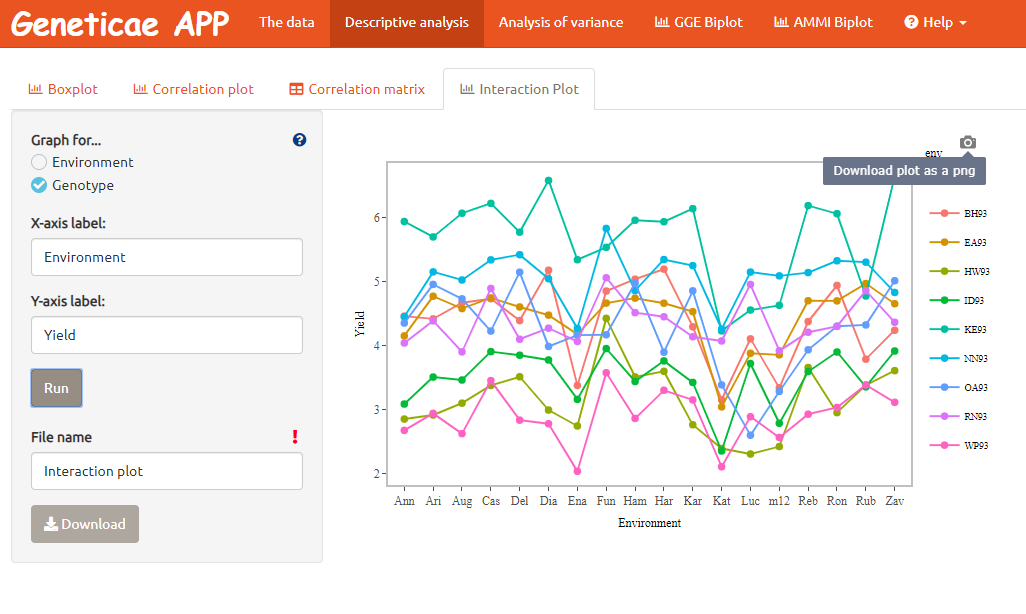
\includegraphics[width=16cm]{./Graficos/int_plot.png}
	\end{center}
	\caption{Boxplot de genotipos a través de los ambientes para el conjunto de datos Plrv}
	\label{fig:figdesc4}
\end{figure}



\textbf{Análisis de la variancia}


La variación fenotípica se puede explicar a partir de los efectos ambienteales, genotípicos y de la interacción entre ambos, cuya significancia se prueba con un ANOVA. Si únicamente los efectos de G y A resultan significativos (es decir, no hay efecto interacción), la interacción debe ser ignorada y los biplots carecen de sentido. En caso de no contar con repeticiones en el conjunto de datos, la interacción no podrá ser testeada y un mensaje aparecerá aclarando lo mencionado \emph{``The interaction effect can be tested since there are repetitions in the data set"}. Por lo tanto, en este caso que no se cuenta con repeticiones, se puede prueba si existe efecto genotípicos y ambienteales (Figura \ref{fig:fig438})

\begin{figure}[H]
	\begin{center}
		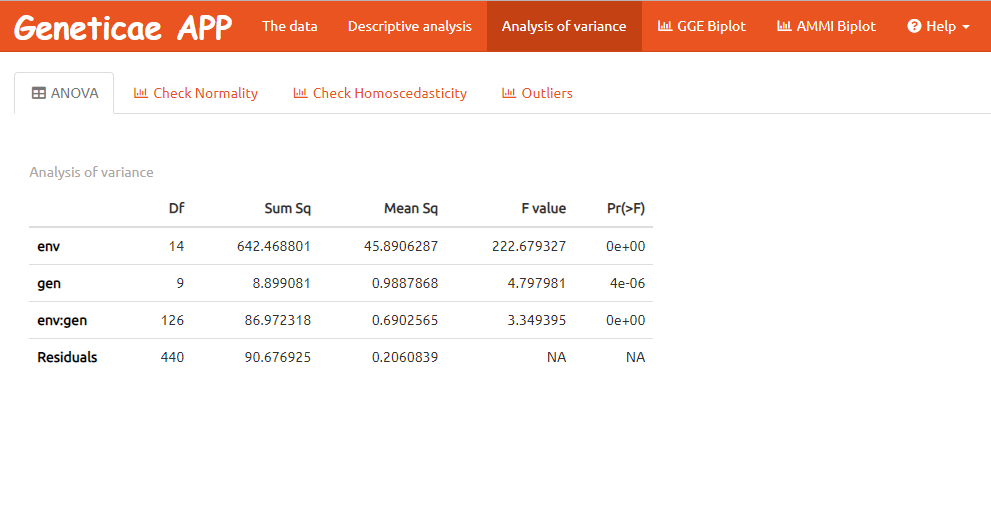
\includegraphics[width=16cm]{./Graficos/ANOVA.png}
	\end{center}
	\caption{Boxplot de genotipos a través de los ambientes para el conjunto de datos Plrv}
	\label{fig:fig438}
\end{figure}


La validez de las conclusiones del ANOVA depende del cumplimiento de que los errores tengan distribución normal con media cero y variancia constante. Tres pestañas de la aplicación: \emph{Check normality}, \emph{Check homocedasticity} y \emph{Outliers} permiten verificar los supuestos mencionados.

El supuesto de normalidad se puede verificar gráficamente con un histograma y un gráfico de probabilidad normal (Figura \ref{fig:fig439}). Además, se puede probar con el test de shapiro-wilks sobre los residuos del ANOVA. Al realizar este test, aparecerá un mensaje con la conclusión del mismo (Figura \ref{fig:fig439}). 

\begin{figure}[H]
	\begin{center}
		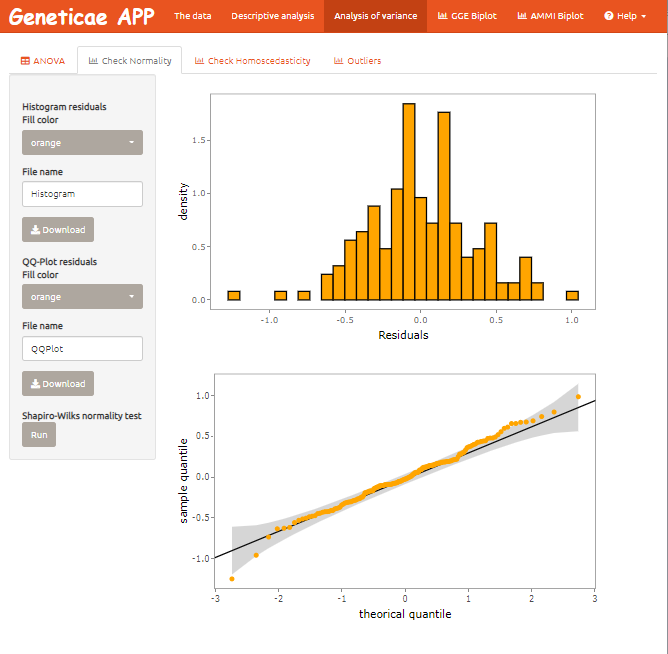
\includegraphics[width=16cm]{./Graficos/Normalidad.png}
	\end{center}
	\caption{Boxplot de genotipos a través de los ambientes para el conjunto de datos Plrv}
	\label{fig:fig439}
\end{figure}


El supuesto de variancia constante u homocedasticidad se puede probar con un gráfico de residuos vs. valores predichos, así como también con el test de levene (Figura \ref{fig:fig4310}). Dicho test se puede verificarr tanto para los genotipos como para los ambientes, y al hacer click en el mismo un mensaje saldrá con la conclusión obtenida del mismo.

\begin{figure}[H]
	\begin{center}
		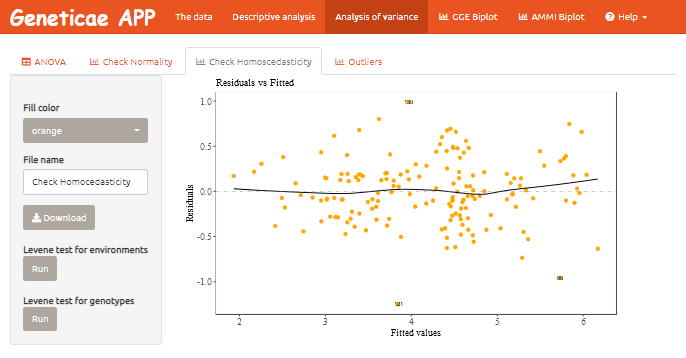
\includegraphics[width=16cm]{./Graficos/Homocedasticidad.png}
	\end{center}
	\caption{Boxplot de genotipos a través de los ambientes para el conjunto de datos Plrv}
	\label{fig:fig4310}
\end{figure}

Por último, el ANOVA no es robusto ante la presencia de observaciones atipicas, por lo tanto se incluyen gráficos para detectar las mismas \ref{fig:fig4311}).

\begin{figure}[H]
	\begin{center}
		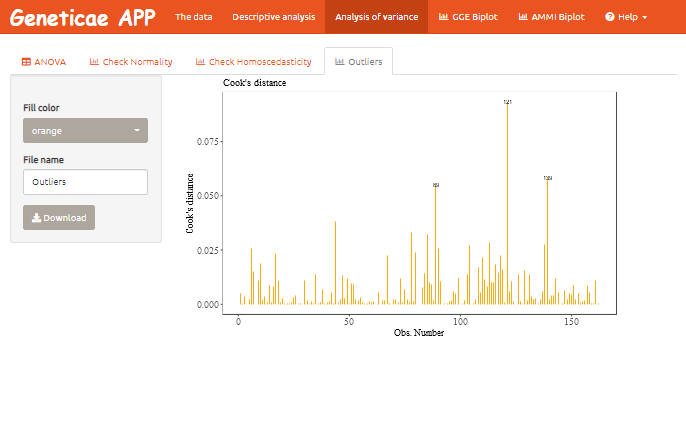
\includegraphics[width=16cm]{./Graficos/Outliers.png}
	\end{center}
	\caption{Boxplot de genotipos a través de los ambientes para el conjunto de datos Plrv}
	\label{fig:fig4311}
\end{figure}

Todos los gráficos mostrados para verificar los supuestos requeridos por la técnica ANOVA pueden ser descargados mediante el botón \emph{Download} de la pestaña correspondiente.

\textbf{Biplots}

\emph{Geneticae Shiny Web App} permite obtener tanto el biplot GGE (Figura \ref{fig:fig4312}) como el GE (Figura \ref{fig:fig4313}) . Ciertos atributos estilísticos de dichos gráficos se pueden personalizar y además pueden ser descargados.

Dada la importancia del biplot GGE, se incluyen aquellos más utilizados en el análisis de datos provenientes de EMA. Entre ellos, el biplot básico y aquellos que permiten estudiar la relación entre los ambientes (\emph{Relationship Among Environments}), la identificación del mejor cultivar en cada ambiente (\emph{Which Won Where/What}), Discrimination vs. representativeness ( \textbf{Este es el q me falta interpretar en el paquete} ), clasificación de los ambientes con respecto al ambiente ideal (\emph{Ranking Environments}), evaluación de los cultivares con base en el rendimiento promedio y la estabilidad (\emph{Mean vs. Stability}) y  clasificación de genotipos con respecto al genotipo ideal (\emph{Ranking Genotypes}). A la hora de indicar el biplot que se desea realizar se debe especificar el método de SVD, centrado y escalado que se desea. Se debe tener en cuenta que no todos los biplots se hacen con el mismo método SVD, para más detalle recurrir a Yan ...\textbf{CITA}.


\begin{figure}[H]
	\begin{center}
		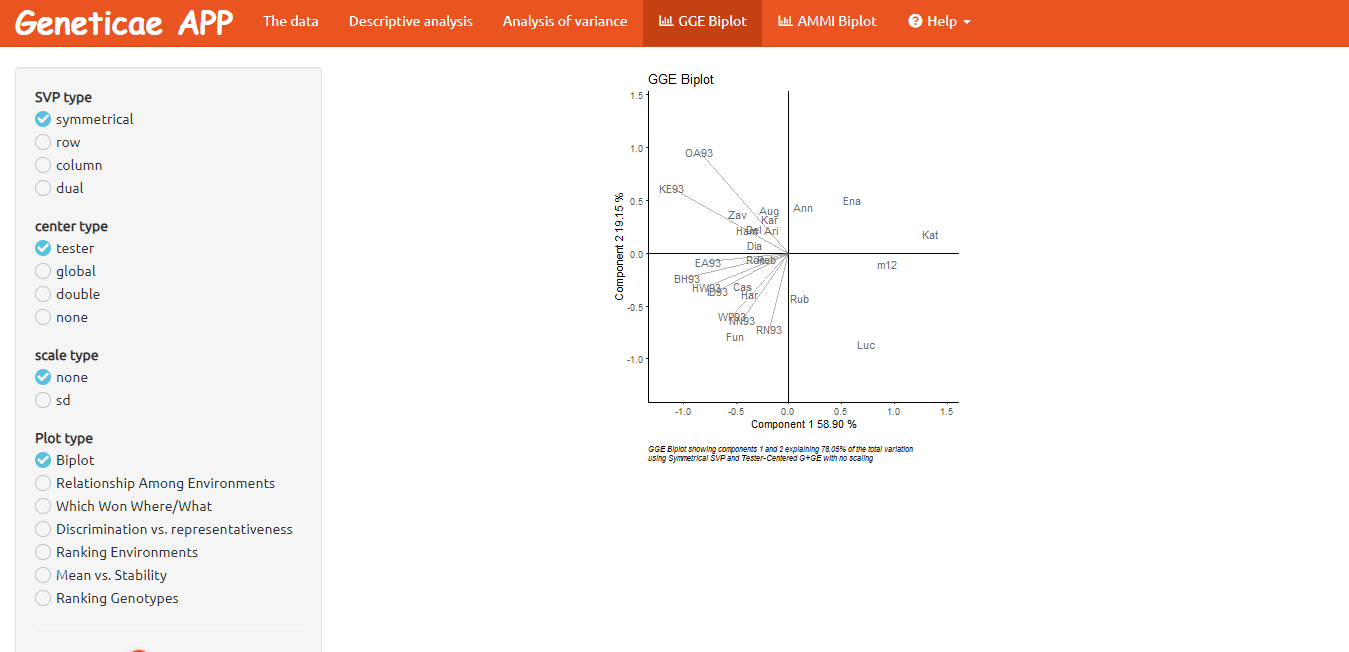
\includegraphics[width=16cm]{./Graficos/GGE.png}
	\end{center}
	\caption{Boxplot de genotipos a través de los ambientes para el conjunto de datos Plrv}
	\label{fig:fig4312}
\end{figure}


\begin{figure}[H]
	\begin{center}
		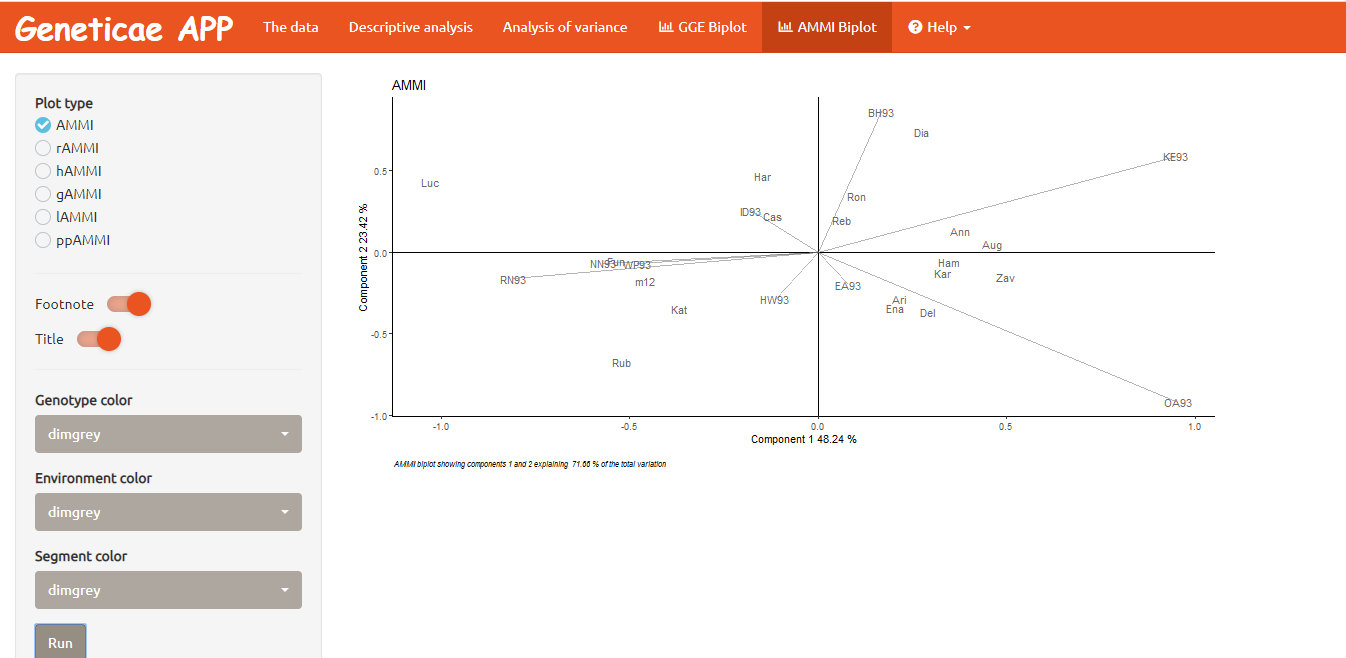
\includegraphics[width=16cm]{./Graficos/AMMI_S.png}
	\end{center}
	\caption{AMMI}
	\label{fig:fig4313}
\end{figure}



\textbf{Ayuda}

Información general y un tutorial de cómo utilizar la aplicación se encuentra disponible en la última pestaña de la misma. Allí se encuentran disponibles ejemplos con una de los conjuntos de ejemplo disponible en la misma.  
